\documentclass{article}
\usepackage[utf8]{inputenc}
\usepackage[english]{babel}
\usepackage[utf8x]{inputenc}
\usepackage[T1]{fontenc}

%% Sets page size and margins
\usepackage[a4paper,top=2.5cm,bottom=2cm,left=2.5cm,right=2.5cm,marginparwidth=1.75cm]{geometry}

%% Useful packages
\usepackage{amsmath}
\usepackage{graphicx}
\usepackage[colorinlistoftodos]{todonotes}
\usepackage[colorlinks=true, allcolors=blue]{hyperref}
\usepackage[draft]{fixme}
\fxsetup{inline,nomargin,theme=color}

\usepackage{lastpage}
\usepackage{fancyhdr}
\headheight = 14 pt
\pagestyle{fancy}
\lhead{VR Proposal 2021}
\chead{ReCognition}
\rhead{Project description}
\lfoot{}
\cfoot{\thepage (\pageref{LastPage})}
\rfoot{}

\usepackage[utf8]{inputenc}
\usepackage{amsmath}
\usepackage{graphicx}

\title{Cognitive Tradeoffs in Learning to Communicate}
\author{Devdatt Dubhashi and Shalom Lappin}
\date{February 2021}

\begin{document}

\maketitle

\section{Introduction}
Although there is a wide diversity of human languages, there are nevertheless some universal similarities underlying all of them e.g. word frequency distributions, syllable durations, word lengths, syntactic structures, and case marking all facilitate efficient communication (see \cite{Regier2015} and references cited therein). Why do languages partition mental concepts in the ways they do?

There is an increasingly influential proposal that language is shaped by the need for \emph{efficient communication} \cite{Kemp2018}, which by its nature involves a trade-off between \emph{simplicity}, which minimizes cognitive load, and \emph{informativeness} which maximizes communicative effectiveness. Specifically, there is a suggestion that good communication schemes achieve a near-optimal trade-off between these constraints as shown schematically in Figure~\ref{fig:opt}.
\begin{figure}
    \centering
    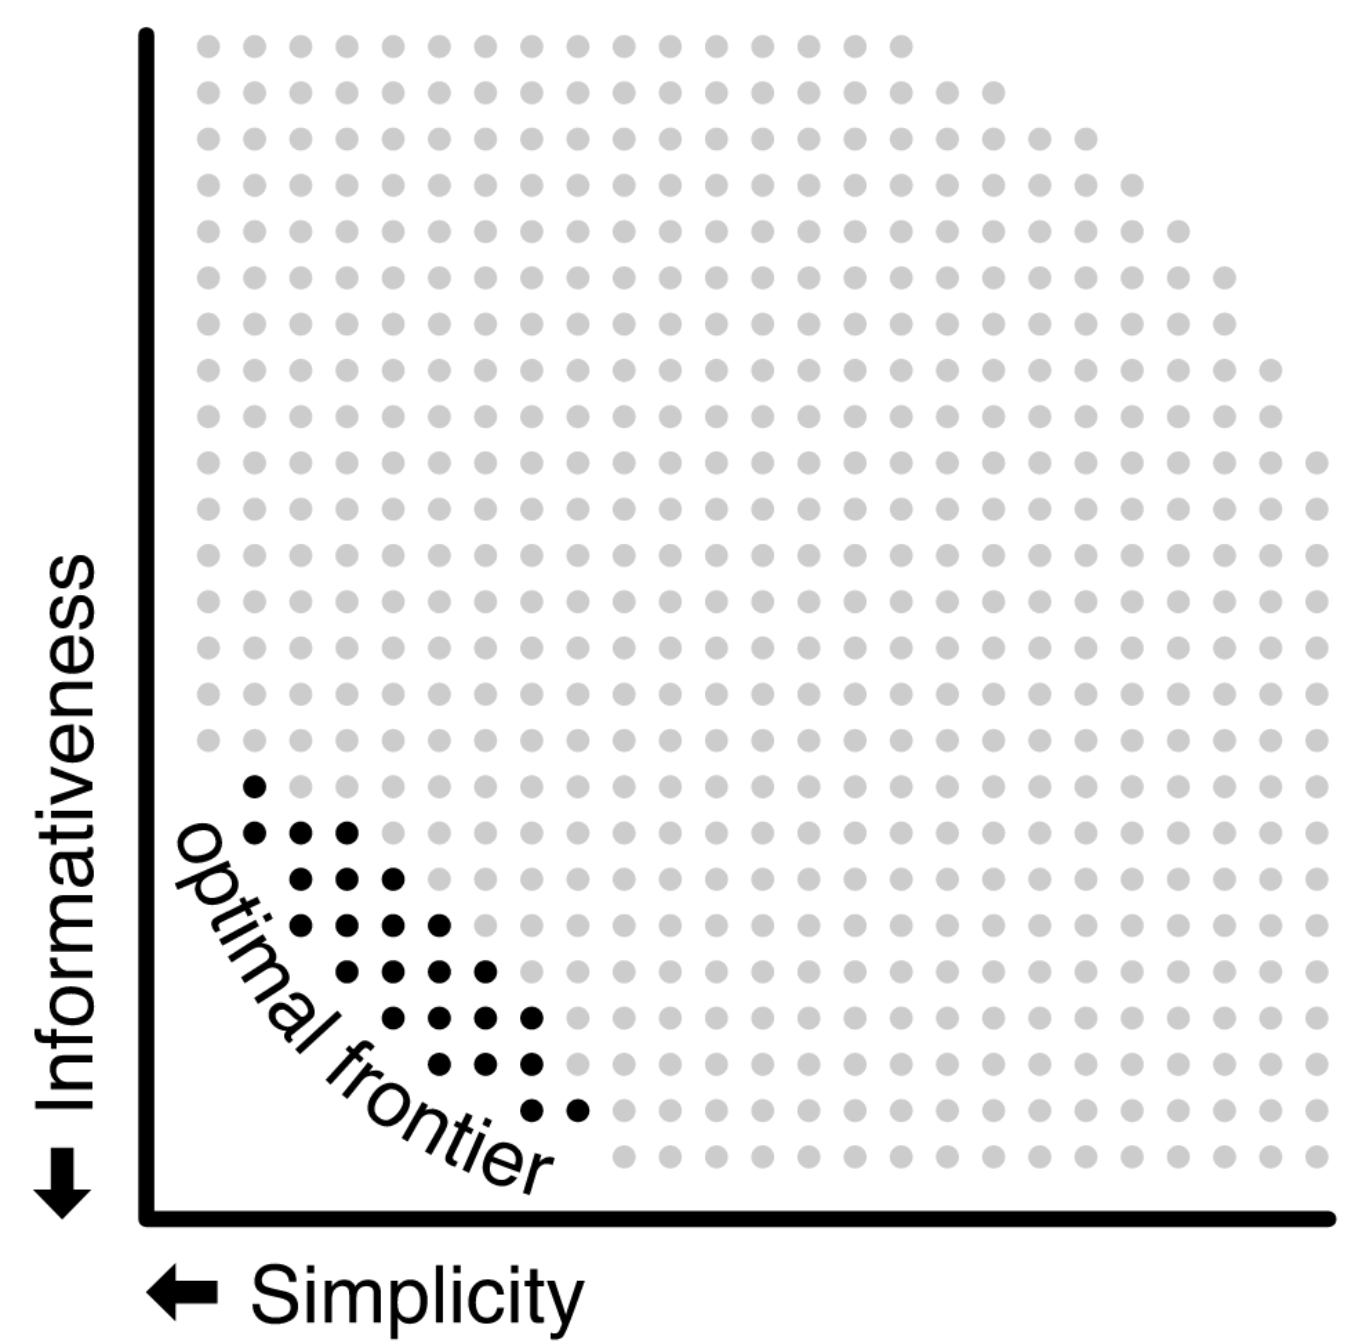
\includegraphics[width=0.42\textwidth]{Figures/fig_optimal_frontier.png}
    \caption{Optimal tradeoff between simplicity and informativeness}
    \label{fig:opt}
\end{figure}

Languages are posited to be designed to facilitate efficient communication between agents. A schematic illustration of the framework is shown in Figure~\ref{fig:regier_model}. The sender has a concept in mind and wishes to convey this to a listener over a discrete communication channel. The listener then tries to reconstruct the concept. The communication scheme or language is designed to optimize the successful reconstruction of the mental concept.
\begin{figure}[t]
\centering
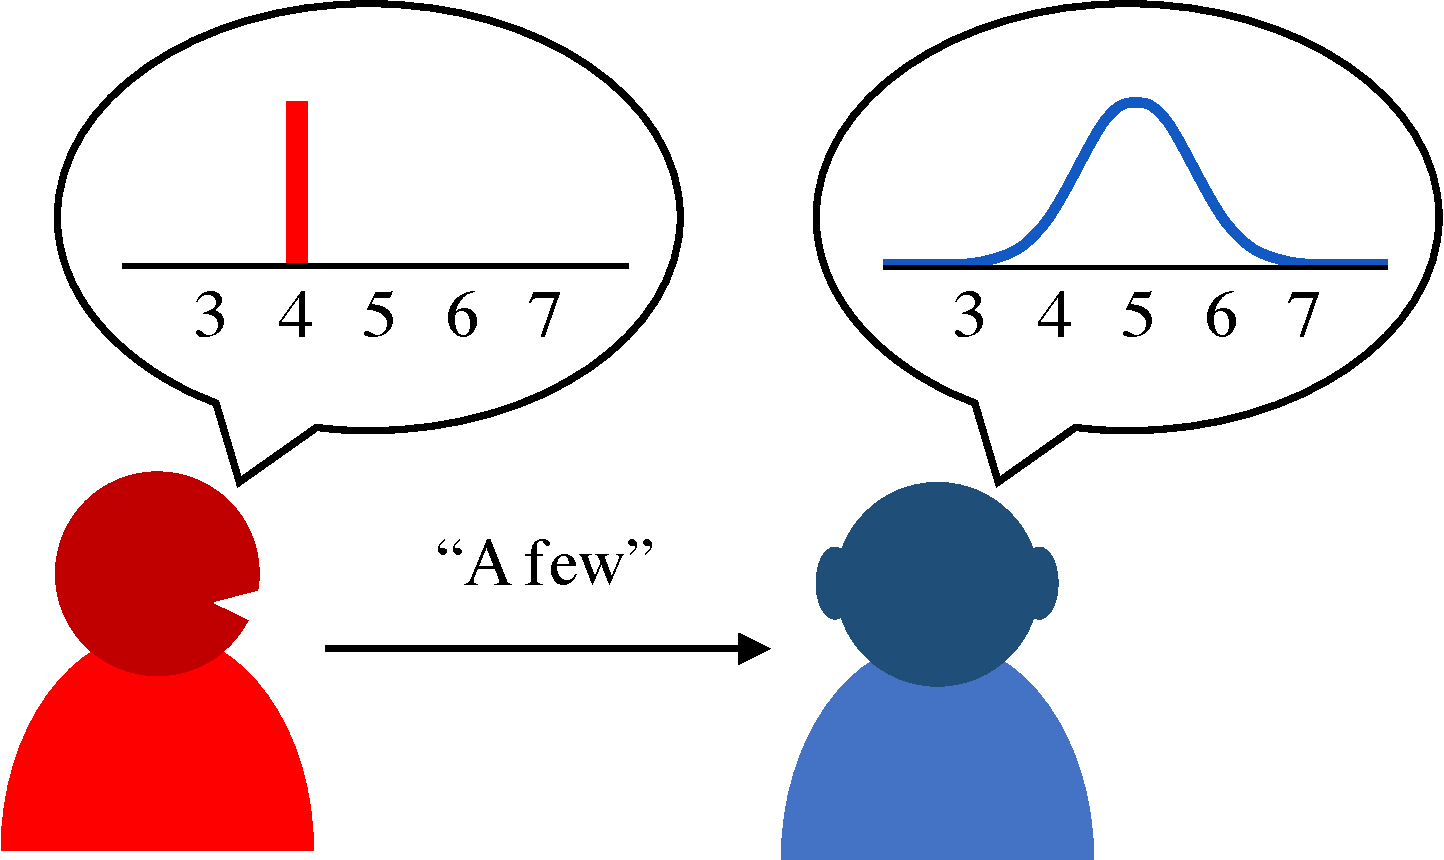
\includegraphics[width=0.42\textwidth]{Figures/regier_model_2.pdf}
\caption{Illustration of the communication setup presented in \citet{Xu2020}. The sender wants to convey the numeral concept $4$ and utters ``a few''. The listener is unsure of which numeral the sender is referring to and produces a probability distribution over possible numerals.}\label{fig:regier_model} 
\end{figure}

This can be couched more precisely in the classic setting  of \emph{Shannon information theory} \cite{CT06} which considers the fundamental laws of transmitting information over a noisy channel, see Figure~\ref{fig:comm} taken from \cite{ZKRT18}.
\begin{figure}
    \centering
    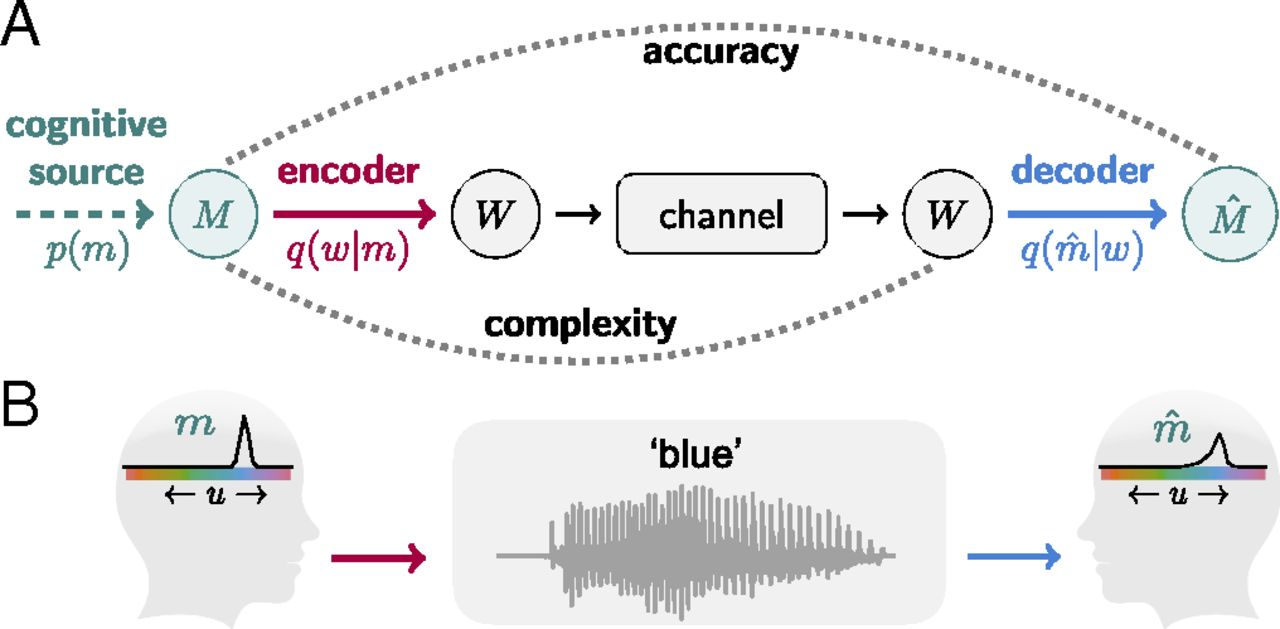
\includegraphics{Figures/comm.jpg}
    \caption{Language as communication over a noisy channel}
    \label{fig:comm}
\end{figure}
In this setting, the source message $M$ and its reconstruction $\hat{M}$̂ are distributions over objects in the universe $U$. $M$ is compressed into a \emph{code word} $W$ which is transmitted over a noisy channel. At the receiver, the reconstruction $\hat{M}$ 
of the source message is based on $W$. The accuracy of communication is determined by comparing $M$ and $\hat{M}$ and the \emph{complexity} of the scheme is determined by the mapping from $M$ to $W$. In (B), this scheme is specialized to communicating colours where $U$ is a set of colors, shown for simplicity along a single dimension. The speaker communicates a specific colour concept $m$ by uttering the word “blue,” and the listener interprets blue as meaning $\hat{m}$. 

The information theoretic view leads naturally to view the symbolic linguistic terms used for the communication as \emph{codes} that create \emph{partitions} of semantic spaces, and has a wide explanatory power across a variety of domains, see the reviews \citet{Kemp2018, Gibson2019}. 


However, a fundamental question that is left unaddressed is to understand this tradeoff between simplicity and informativenss of the communication scheme in a \emph{quantitative computational} way
\begin{eqnarray}
  \label{eq:fund}  
  \mbox{What are the computational tradeoffs in learning efficient commnuncation schemes?} \nonumber \\
  \mbox{How are they reflected in the resulting communication schemes?}
\end{eqnarray}
 
For example, it has been shown recently that numeral systems across languages reflect a need for efficient communication \citep{Xu2020}. Numeral systems come in many shapes, some are recursive like English and can express any numeriosity while other non-recursive systems only consists of a small set of words \citep{wals-131}. These non-recursive systems could be either \emph{exact restricted} - in the sense that exact numerosities can only be expressed on a restricted range, or \emph{approximate} like in the language Mundurukú where most numeral words have an imprecise meaning \citep{Pica2004}. Could we explain these different numeral systems computationally as the result of tradeoffs  between simplicity and informativenss along the optimal frontier in Figure~\ref{fig:opt}? For instance, could a computational system has limited computing capability but large memory lead to the direct encoding systems whereas one with more flexible computing but limited memory lead to compavct recursive systems?


\subsection{Reinforcement Learning Approach to Cognitive Science} 
Here we outline an approach that addresses the fundamental question (\ref{eq:fund}) via reinforcement learning (RL). 
%\cite{SB18,F-L18}. 
There is an increasing realization that RL may offer more than just a computational theory for affective decision-making but that RL algorithms appear to be directly instantiated in human cognition e.g. 
learning algorithms seem to be centrally implicated in exploration strategies used by humans \citep{Wilson2014, Schulz2019, Eckstein20}. 

The availability of a growing suite of environments (from simulated robots to Atari games), toolkits, and sites for comparing and reproducing results about RL algorithms applied to a variety of tasks makes it possible to study cognitive science questions through a different lens using RL. If simple RL algorithms are indeed a good proxy for actual human learning, then insights about questions of universals in language learning could be obtained very cheaply and reliably via controlled experiments in such \emph{in silico} settings. Our approach could be used to explore various trade-offs at the heart of efficient communication. 


\section{Significance and Scientific Novelty}
This proposal addresses questions at the heart of cognitive science, linguistics and AI/machine learning. The question we ask can be illuminatingly posed in the framework of Marr's three levels of analysis \cite{Marr82} proposed in the context that complex systems such as the brain, a computer or human behaviour should be understood at different levels. Marr's framework proved to be an elegant and popular way of reasoning about complex systems, and in the context of machine learning and statistics. Marr's three levels framework consists of:
\begin{description}
\item[Computational]
We describe and specify the problems we are faced with in a generic manner, but do not say how these problems are to be solved. 
\item[Algorithmic]
This level forms a bridge between the computational and implementational levels, describing how  the identified computational problems can be solved. 
\item[Implementational]
The physical substrate or mechanism, and its organisation, in which computation is performed. This could be biological in the case of neurons and synapses, or in silicon using transistors, etc.
\end{description}

\section{Project Description}
\subsection{Neural Turing Machines}
Deep neural networks are remarkably adept at supervised learning and reinforcement learning, but are limited in their ability to represent variables and data structures and to store data over long timescales, owing to the lack of an external memory. Recent work has introduced a hybrid model, the \emph{a differentiable neural computer} (DNC) \cite{graves2014neural, DNC}, which consists of a neural network that can read from and write to an external memory matrix, analogous to the random-access memory in a conventional computer. Like a conventional computer, it can use its memory to represent and manipulate complex data structures, but, like a neural network, it can learn to do so from data. Analogies can be made between the external memory in these models and the human working memory. Thus, the DNC offers a convenient and flexible computational framework to study cognitive capacity tradeoffs. So examples are...

\section{Preliminary Results}

\section{National and International Collaborations}

Terry Regier expressed strong interest.

\section{Equipment and Infrastrucure}


\bibliographystyle{abbrv}
\bibliography{refs}
\end{document}

